\chapter{Návrh modelu}\label{chap:proposal}

V tejto kapitole si opíšeme cieľ diplomovej práce, zameriame sa na návrh modelu všetkých častí aplikácie a definujeme si požiadavky na ich funkcionalitu. 

\section{Cieľ práce}
\begin{itemize}
	\item Navrhnúť prostredie grafického editora
	\item Implementovať grafický editor do prostredia MediaWiki pomocou rozšírenia
	\item Navrhnúť a implementovať spôsob ukladania verzií výstupných súborov grafického editora
	\item Navrhnúť a implementovat komunikačný protokol na synchronizáciu grafického editora pre viacero nezávislých používateľov
	\item Integrovať rozšírenie s webovou stránkou fakulty http://wiki.matfyz.sk
\end{itemize}

\section{Návrh riešenia}
Riešenie diplomovej práce bude pozostávať z dvoch hlavných častí. Prvo časťou bude navrhnutie synchronizačného servera, ktorý bude zabezpečovať výmenu informácií medzi klientmi. V druhej časti navrhneme samotný grafický editor obrázkov. Vysvetlíme si spôsob integrácie editora do systému MediaWiki a popíšeme si jeho požadované vlastnosti.

\subsection{Požiadavky na synchronizačný server}\label{sec:poziadavky_na_server}
Synchronizačný server bude pozostávať z aplikácie naprogramovanej v jazyku JavaScript. Spúšťaný bude v runtime prostredí NodeJS. Primárnou úlohou bude zaradiť pripojeného používateľa do miestnosti zodpovedajúcej editovanému súboru, vďaka čomu zabezpečíme synchronizáciu údajov medzi všetkými používateľmi pracujúcimi s týmto súborom. Využijeme pri tom knižnicu Socket.IO, konkrétne jej serverovú verziu, ktorá bude slúžiť ako hlavný komunikačný protokol postaveného na báze WebSocket protokolu. Aplikácia synchronizačného servera bude pozostávať z niekoľkých entít (objektov), ktoré si postupne popíšeme v ďalších častiach tejto diplomovej práce.

\subsubsection{Popis základných entít synchronizačného servera}
\paragraph{Entita User}

Základnou entitou bude objekt \textit{User}, ktorý definuje vlastnosti pripojeného používateľa. Medzi informácie uchovávané v tomto objekte budú patriť \textit{meno}, jeho zodpovedajúca \textit{farba} kurzora, pod ktorou bude rýchlo rozpoznateľný inými používateľmi a \textit{jedinečný identifikátor} získaný po pripojení na server.

\paragraph{Entita Message}
Editor bude poskytovať možnosť textovej komunikácie medzi používateľmi. Kvôli tomu je potrebné navrhnúť objekt reprezentujúci takúto správu. Medzi jeho vlastnosti bude patriť informácia, kto správu odoslal, pre koho je určená, čas kedy bola odoslaná a taktiež textový obsah správy. Pre potreby lepšej informovanosti o stave pripojených používateľov bude možné odosielať takzvanú systémovú správu, ktorá bude určená pre všetkých používateľov.

\paragraph{Entita Object}
Informácie o objektoch grafickej plochy budeme synchronizovať pomocou JavaScriptového objektu typu \textit{Object}. Bude to objekt dynamickej štruktúry s niekoľkými základnými vlastnosťami. Tými sú \textit{jedinečný identifikátor objektu}, informácia o \textit{stave uzamknutia} a v prípade uzamknutého objektu taktiež informácia o \textit{používateľovi, ktorý daný objekt uzamkol}. Ďalšie informácie o objekte sú závislé od jeho dátového typu generovaného na klientskej strane grafického editora.

\paragraph{Entita Room}
Každý používateľ bude po pripojení na synchronizačný server automaticky zaradený do miestnosti zodpovedajúcej editovanému súboru. Táto miestnosť bude reprezentovaná objektom Room s vlastnosťami popisujúcimi jej aktuálny stav. Bude sa tu nachádzať zoznam pripojených používateľov, zoznam odoslaných správ, zoznam grafických objektov editora, informáciu o formáte editovaného súboru a vlastnostiach grafickej plochy.

\paragraph{Entita RoomManager}
Aby sa predišlo zbytočnému udržiavaniu stavov miestností v ktorých sa nenachádzajú žiadni používatelia, musíme navrhnúť entitu, ktorá bude riadiť dynamické vytváranie a odstraňovanie miestností. Pre tento účel vytvoríme objekt RoomManager, ktorý bude obsahovať zoznam všetkých miestností a funkcie na vytvorenie miestnosti pri pripojení prvého používateľa a jej vymazanie v prípade že sa z nej odpojil posledný používateľ.

\subsubsection{Funkčné požiadavky synchronizačného servera}

\begin{itemize}
	\item \textbf{Pripojenie používateľa} - vytvorí sa objekt typu \code{User} a nastavia sa mu vlastnosti na základe zaslaného dopytu. 
	
	\item \textbf{Overenie pripojeného používateľa} - po pripojení používateľa sa overí správnosť overovacieho tokenu. Ak overovací token nie je správny, používateľ nebude mať umožnené pripojenie do zvolenej miestnosti.
	
	\item \textbf{Vytvorenie miestnosti} - v prípade, ak sa pripojený používateľ má zaradiť do miestnosti ktorá aktuálne neexistuje, takáto miestnosť je vytvorená a následne je do nej používateľ zaradený. V prípade že daná miestnosť už je vytvorená, používateľ sa do nej zaradí automaticky a táto informácia sa odošle všetkým ostatným používateľom nachádzajúcim sa v miestnosti.
	
	\item \textbf{Synchronizácia editora} - po pripojení a zaradení používateľa do miestnosti zodpovedajúcej editovanému súboru, bude server schopný prijímať synchronizačné správy o zmenách vykonaných používateľom v prostredí editora. 
	
	Pri \textit{vytvorení nového grafického objektu} editora sa odosiela požiadavka s informáciami o tomto objekte na synchronizačný server. Ten požiadavku spracuje, pridá objekt do zoznamu objektov na základe jeho jedinečného identifikátora a odošle informáciu o novom objekte všetkým ostatným používateľom pripojeným do miestnosti.
	
	\textit{Modifikáciou existujúceho grafického objektu} editora bude taktiež odoslaný dopyt o tejto akcii synchronizačnému server. Ten ho spracuje, zmení zodpovedajúci objekt na základe prijatých informácií a odošle správu o zmene objektu spolu so zmenenými údajmi všetkým ostatným používateľom.
	
	Ak je objekt v grafickom editore odstránený, táto akcia bude taktiež odoslaná na synchronizačný server spolu s jedinečným identifikátorom objektu. Ten ho spracuje, odstráni zodpovedajúci objekt zo zoznamu a následne odošle ostatným používateľom informáciu o vymazaní tohoto objektu.
	
	Aby sa predišlo konfliktom pri zmenách vlastností objektov, je potrebné navrhnúť proces ich automatického uzamykania. To zabezpečíme tak, že pri zvolení aktívneho objektu v grafickom editore, bude odoslaná požiadavka na jeho uzamknutie daným používateľom na server. Táto akcia je znova synchronizovaná so zvyšnými editormi používateľov. V prípade že objekt už uzamknutý bol, odošle sa odpoveď o zamietnutí uzamknutia objektu.
	
	\item \textbf{Odpojenie používateľa} - pri tejto akcií je potrebné vykonať niekoľko úkonov. Najskôr musia byť odomknuté všetky objekty, ktoré boli uzamknuté týmto používateľom a následne sa odstráni z miestnosti. V prípade že miestnosť zostane prázdna, vymaže sa. Inak je odoslaná informácia o odpojení používateľa všetkým zvyšným pripojeným klientom.
	
	\item \textbf{Odstránenie miestnosti} - ako sme spomenuli vyššie, miestnosť bude automaticky odstraňovaná pri odchode posledného používateľa.
	
\end{itemize}

\subsection{Editor obrázkov}
Grafický editor bude implementovaný formou MediaWiki rozšírenia, naprogramovaného primárne v jazyku JavaSrcipt, s použitím frameworku AngularJS. Na komunikáciu so synchronizačným serverom použijeme JavaScriptovú knižnicu Socket.IO, konkrétne jej klientskú verziu. 

\subsubsection{Funkčné požiadavky grafického editora}
\begin{itemize}
	\item \textbf{Výber nástroja} - grafický editor bude poskytovať viacero pracovných nástrojov na vytváranie rôznych typov grafických objektov. Tie bude možné zvoliť kliknutím na ikonu reprezentujúcu zvolený nástroj. 
\end{itemize}


\begin{figure}[h]
	\centerline{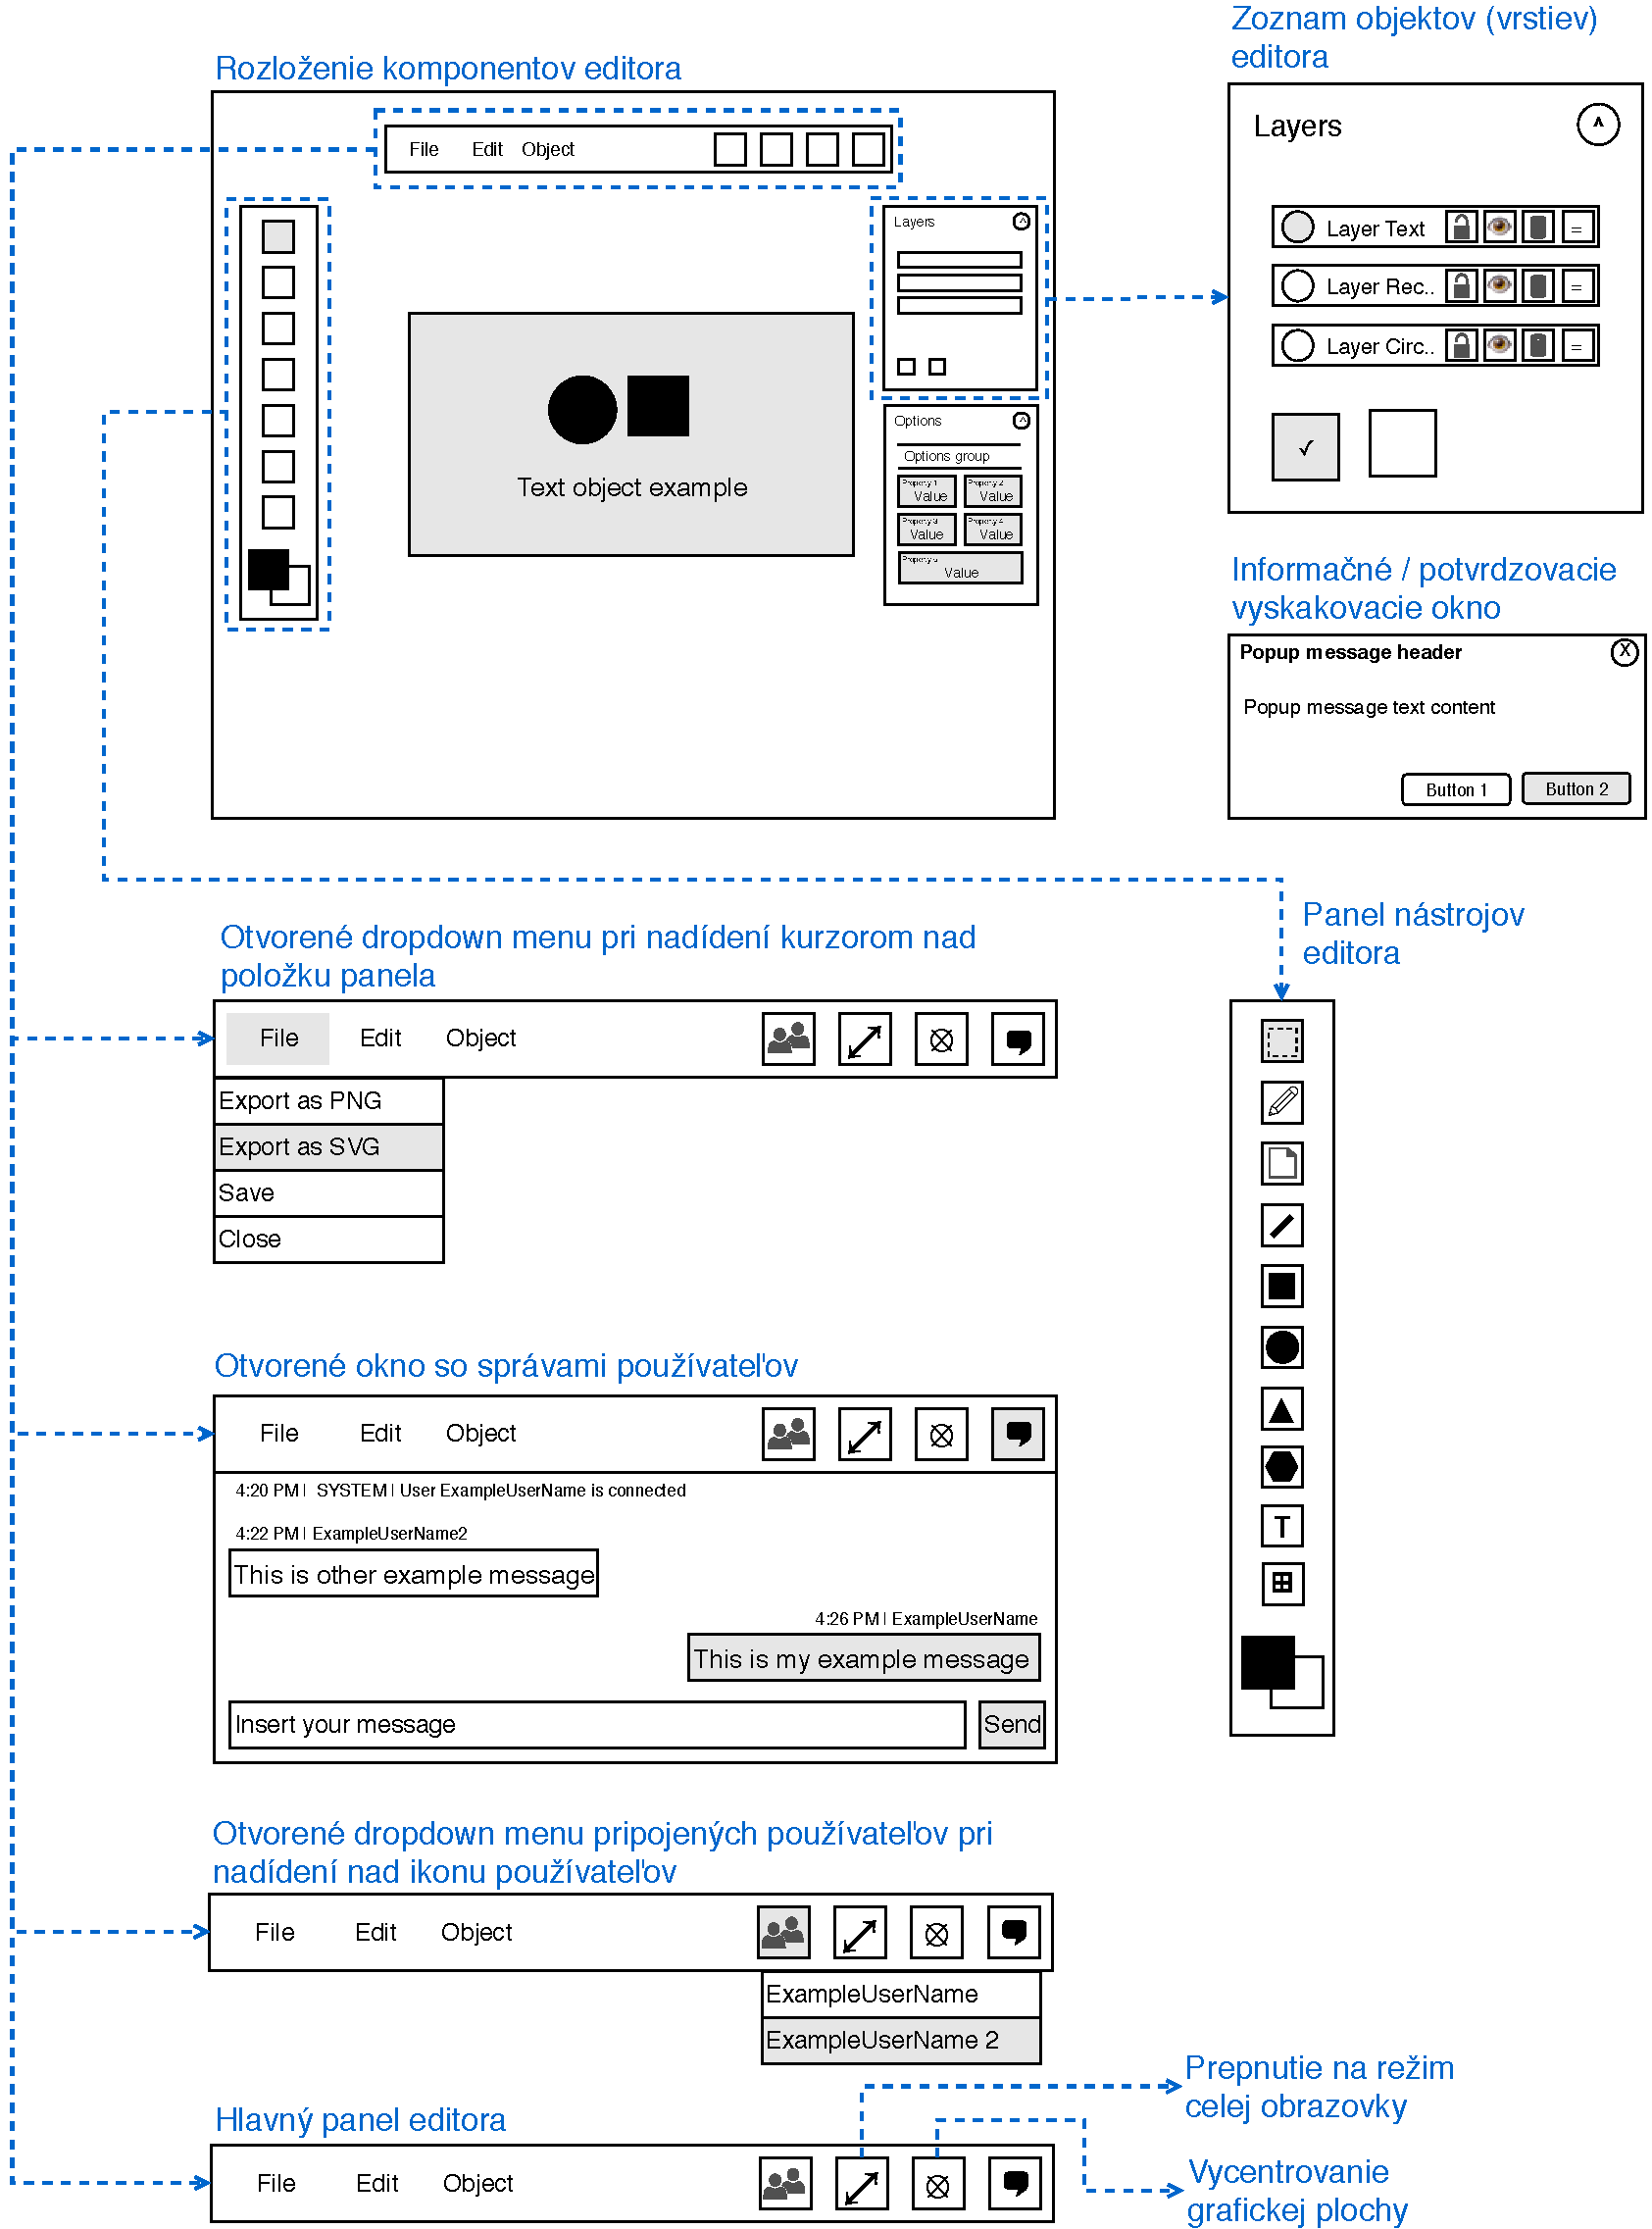
\includegraphics[width=1\textwidth]{images/diagrams/editor_wireframe_base}}
	\caption[Rozloženie komponentov editora]{Návrh rozloženia komponentov používateľského prostredia editora}
	\label{obr:editor_wireframe_base}
\end{figure}
\FloatBarrier

\subsubsection{Integrácia do sytému MediaWiki}
% TODO: popisat akym sposobom bude editor integrovany do mw, preco special page, atd.